\section{Problem 1}

\subsection{} %1.1

Since the solid cone $\cQ^3$ is closed, convex,
and rotational symmetric along the first axis ($t$ axis),
we only need consider a small set $S$ of candidate points
when trying to find the projection of a point $y$ into this set $\cQ^3$.
This is because the point projected to must be unique
and thus we can eliminate points that have `brother/sister' points which
shares the same distance to $y$ due to symmetry.
Specifically, we can choose $S$ be the (or a) plane that contains
both the point $y$ and the first axis.
The problem then reduces to a simple two-dimensional geometry problem
of middle school level (Figure~\ref{fig:1}).
We can directly write down the solution as specified in the question.

\begin{figure}[ht]
\centering
    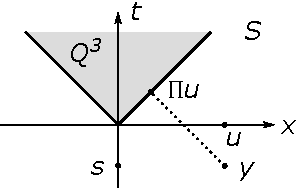
\includegraphics[width=0.36\linewidth]{figure/fig1}
    \caption{\small
    The problem of projecting point $y=(t,u)$ to $\cQ^3$ is
    reduced to this two dimensional problem.}
    \label{fig:1}
\end{figure}

\subsection{} %1.2

Let point $z=\Pi_H(y)=(a,b,a)\in H$ be the projected point.
Then $z-y=(a-s, b-u_1, a-u_2)$ must parallel to the normal direction of plane $H$,
which is $n=(1,0,-1)$.
Solve this constraint,
we get $b=u_1$ and $a=(s+u_2)/2$.
